
% In this section we go over related work and relevant background information for our model and experiments. The depth of the explanation is adopted to the expected prior knowledge of the reader. The reader is supposed to know the basics of machine learning and deep learning, including probability theory and basic knowledge on neural networks and their different architectures. Basic principles such as forward pass, backpropagation and convolutions are expected to be understood. Further the use and functionality of deep learning modules such as the model, the optimizer and the terms target and prediction should be known. This also includes being familiar with the training and testing pipeline of deep learning.

This section derives and explains the techniques, which form the backbone of this research. For fundamental background on machine learning and probability theory we refer the reader to Bishops book \cite{bishop_pattern_2006}. We begin with introducing the VAE and its differences to a normal autoencoder. Further we show how convolutional layers can act on graphs and how these layers can be used in an encoder model, the GCN. Building on these modules, we present the main model for this thesis, the Relational Graph VAE (RGVAE). Finally, we present a popular graph matching algorithm, which is intended to match prediction and target graph \cite{paulheim_knowledge_2016}.  


\subsection{Knowledge Graph}

% Knowledge Graphs are great! The best in the world.
% Knowledge Graphs which we be using
% We focus on the generation of KGs.
% Representation of KG as adjacency, edge feature and node feature matrix
'Knowledge graph' has become a popular term. Yet, the term is so broad, that its definitions varies depending on domain and use case \cite{ehrlinger2016towards}. In this thesis we focus on KGs in the context of relational machine learning.

% What is a KG
Both datasets of this thesis are derived from large-scale KG data in RDF format. The Resource Description Framework (RDF), originally introduced as infrastructure for structured metadata, is used as general description framework for the semantic-web applications \cite{miller1998introduction}. It involves a schema-based approach, meaning that every entity has a unique identifier and possible relations limited to a predefined set. The opposite schema-free approach is used in OpenIE models, such as AllenNLP \cite{gardner_allennlp_2018}, for information extraction. These models generate triples from text based on NLP parsing techniques which results in an open set of relations and entities. In this thesis a schema-based framework is used and triples are denote as $(s,r,o)$. A exemplar triple from the FB15K-237 dataset is


\begin{center}
    \texttt{/m/02mjmr, /people/person/place\_of\_birth, /m/02hrh0\_}.
\end{center}



A human readable format of the entities is given by the \textit{id2text} translation of Wikidata \cite{vrandevcic2014wikidata}.

\begin{itemize}
    \item Subject $s$:   \texttt{/m/02mjmr Barack Obama}
    \item Relation/Predicate $r$:    \texttt{/people/person/born-in}
    \item Object $o$:     \texttt{/m/02hrh0\_ Honolulu}
\end{itemize}


For all triples, $s$ and $o$ are part of a set of entities, while $r$ is part of a set of relations. This is sufficient to define a basic KG \cite{nickel_review_2016}.

% Hierarchy, entities, classes
Schema-based KG can include type hierarchies and type constraints. Classes group entities of the same type together, based on common criteria, e.g. all names of people can be grouped in the class 'person'. Hierarchies define the inheriting structure of classes and subclasses. Picking up our previous example, 'spouse' and 'person' would both be a subclass of 'people' and inherit its properties. At the same time the class of an entity can be the key to a relation with type constraint, since some relations can only be used in conjunction with entities fulfilling the constraining type criteria.

% Ontology - semantics
These schema based rules of a KG are defined in its ontology. Here properties of classes, subclasses and constraints for relations and many more are defined. Again, we have to differentiate between KGs with open-world or closed-world assumption. In a closed-world assumption all constraints must be sufficiently satisfied before a triple is accepted as valid. This leads to a huge ontology and makes it difficult to expand the KG. On the other hand open-world KGs such as Freebase, accept every triple as valid, as long as it does not violate a constrain. This again leads inevitably to inconsistencies within the KG, yet it is the preferred approach for large KGs. In context of this thesis we refer to the ontology as semantics of a KG, we research if our model can capture the implied closed-world semantics of an open-world KG \cite{nickel_review_2016}.

% % Sparse and dense representation
% Lastly, we point out one major difference between KGs, namely their representation. RDF KGs are represented as set of triples, consisting of a unique combination of numeric indices. Each index linking to the corresponding entry in the entity and relation vocabulary. This is called dense representation and benefits from fast computation due to an optimized use of memory.

% In contrary the dense representation of a triple is the sparse representation. Here a binary square matrix also called the adjacency matrix, indicates a link between two entities. To identify the node, each node in the adjacency matrix has a one-hot encoded entity-vocabulary vector. All one-hot encoded vectors are concatenated to a node attribute matrix.
% In simple cases, like citation networks this is a sufficient representation. In the case of Freebase, we need an additional edge-attribute matrix, which indicates the relation  of each link. The main benefit of this method is the representation of subsets of triples, also referred to as subgraphs, with more than one relation and the possibility to perform graph convolutions. 

% Usecases of KG

% Knowledge graphs have very different formats. The datasets we be sorting with are in rdf format.
% This format can include an defined onthology or not.
% This means the KG consists of triples subject, relation, object.
% when indexing these triples. we get a dense representation of the KG.
% About sparse KGs

\subsection{Graph VAE}

Since the graph VAE is a adaptation of the original VAE, we start by introducing the original version, which is unrelated to graph data. Furthermore we present each of the different modules, which compose the final model. This includes the different graph encoders as well as sparse graph loss functions. We define the notation upfront for this chapter, which touches upon three different fields. For the VAE and MLP we consider data in vector format. A bold variable denotes the full vector, e.g. $\mathbf{x}$ and variable with index denotes the element at that index, e.g. for the vector element at index $i$ we denote $x_i$. Graphs are represented in matrices, which are denoted in capital letters. $A$ typically denotes the adjacency matrix, from there on paths split and we use different notations for different methods. While $X$ is described as feature matrix, we have to specify further when it comes to Simonovsky's GraphVAE, where $E$ is the edge attribute and $F$ the node attribute matrix. The reason we change from features to attributes, is due to the singularity, also one-hot encoding of attributes per node/edge, in contrast to features which can be numerous per node.


\subsubsection{VAE}
\label{ssection:VAE}
% The VAE as first presented by \cite{kingma_auto-encoding_2014} is an unsupervised generative model consisting of an encoder and a decoder. The architecture of the VAE differs from a common autoencoder by having a stochastic module between encoder and decoder. Instead of directly using the output of the encoder, a distribution of the latent space is predicted from which we sample the input to the decoder. The reparameterization trick allows the model to be differentiable. By placing the sampling module outside the model we get a deterministic model which can be backpropagated.



The VAE as first presented by \cite{kingma_auto-encoding_2014} is an unsupervised generative model in the form of an autoencoder, consisting of an encoder and a decoder. Its architecture differs from a common autoencoder by having a stochastic module between encoder and decoder. The encoder can be represented as recognition model with the probability $p_{{\theta}}(\mathbf{z} \mid \mathbf{x})$ with $x$ being the variable we want to inference and $z$ being the latent representation given an observed value of $x$. The encoder parameters are represented by $\theta$. Similarly, we denote the decoder as $p_{{\theta}}(\mathbf{x} \mid z)$, which given a latent representation $z$ produces a probability distribution for the possible values, corresponding to the input of $x$. This is the base architecture of all our models in this thesis.

The main contribution of the VAE is to be a stochastic and fully backpropagateable generative model. This is possible due to the reparametrization trick. Sampling from the latent prior distribution, creates stochasticity inside the model, which can not be backpropagated and makes training of the encoder impossible. By placing the stochastic module outside the model, it becomes fully backpropagatable. We use the predicted encoding as mean and variance for a Gaussian normal distribution, from which we then sample $\epsilon$, which acts as external parameter and does not need to be backpropagated and updated.

\begin{figure}[h]
    \centering
    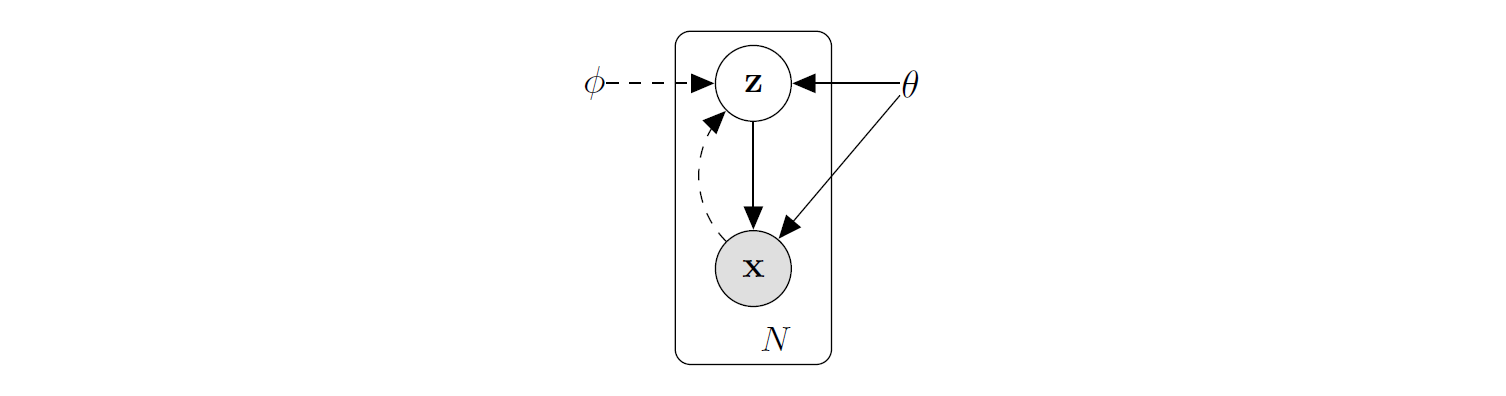
\includegraphics[width=0.75\textwidth]{data/images/repaTrick.png}
    \caption{Representation of the VAE as Bayesian network, with solid lines denoting the generator $p_{{\theta}}(z)p_{{\theta}}(\mathbf{x} \mid z)$ and the dashed lines the posterior approximation $q_{\phi}(\mathbf{z} \mid \mathbf{x})$ \cite{kingma_auto-encoding_2014}.}
    \label{fig:varinference}
\end{figure}

Figure \ref{fig:varinference} shows, that the true posterior $p_{{\theta}}(\mathbf{z} \mid \mathbf{x})$ is intractable. To approximate the posterior, we assume a Standard Gaussian prior $p(\boldmath{z})$ with a diagonal covariance, which gives us the approximated posterior

\begin{equation}
    \log q_{\phi}\left(\mathbf{z} \mid \mathbf{x}\right)=\log \mathcal{N}\left(\mathbf{z} ; \mu(\mathbf{x}), \sigma(\mathbf{x})^{2} \mathbf{I}\right) .
\end{equation}
    
Now variational inference can be performed, which allows both $\theta$ the generative and $\phi$ the variational parameters to be learned jointly. Using Monte Carlo estimation of $q_{\phi}(\mathbf{z} \mid x_1)$ we get the variational estimated lower bound (ELBO)

% Monte Carlo estimate implies ----> only one sample, cuz we sample!

\begin{equation}
    \mathcal{L}\left({\theta}, {\phi} ; x_i\right)=-D_{K L}\left(q_{{\phi}}\left(\mathbf{z} \mid x_i\right) \| p_{{\theta}}(\mathbf{z})\right)+\mathbb{E}_{q_{\phi}\left(\mathbf{z} \mid x_i\right)}\left[\log p_{{\theta}}\left(x_i} \mid \mathbf{z}\right)\right] .
    \label{eq3:elbo}
\end{equation}

We call the first term the regularization term, as it encourages the approximate posterior to be close to the Gaussian normal prior. This term can be integrated analytically and does not require an estimation. The KL-divergence is a similarity measure between two distributions, resulting in zero for two equal distributions. Thus, the model gets penalized for learning a encoder distribution $p_{{\theta}}(\mathbf{z} \mid \mathbf{x})$ which is not Standard Gaussian.

Higgins \textit{et al.} present a constrained variational framework, the $\beta$-VAE \cite{higgins_beta-vae_2016}. This framework proposes an additional hyperparameter $\beta$ which acts as factor on the regularization term. The new ELBO including $\beta$ is

\begin{equation}
    \mathcal{L}\left({\theta}, {\phi} ; \x_i\right)=-\beta \left(D_{K L}\left(q_{{\phi}}\left(\mathbf{z} \mid \x_i\right) \| p_{{\theta}}(\mathbf{z})\right)\right)+\mathbb{E}_{q_{\phi}\left(\mathbf{z} \mid \x_i\right)}\left[\log p_{{\theta}}\left(\x_i} \mid \mathbf{z}\right)\right] .
    \label{eq3:elboBeta}
\end{equation}

For $\beta = 0$ the original VAE is restored and for $\beta>0$ the influence of the regularization term on the ELBO is emphasized. Thus the model prioritizes to learn the approximate posterior $p_{{\theta}}(\mathbf{z} \mid \mathbf{x})$ even closer to the Standard Gaussian prior. In the literature this results in a disentanglement of the latent space qualitatively outperforms the original VAE in representation learning of image data.

The second term represents the reconstruction error, which requires an estimation by sampling. This means using the decoder to generate samples from the latent distribution. In the context of the VAE, these probabilistic samples are the models output, thus, the reconstruction error the similarity between prediction and target\cite{kingma_auto-encoding_2014}.

Once the parameters $\phi$ and $\theta$ of the VAE are learned, the decoder can be used on its own to generate new samples from $p_{{\theta}}(\mathbf{x} \mid z)$. Conventionally, a latent input signal is sampled from $\mathbb{N^{d_z}}$ with $d_z$ being the latent dimension. In the case of discrete binary data, each element of the generated sample is used as probability parameter $p$ for a Bernoulli $\mathbb{B}(1,p)$, from which the final output is sampled. In the case of categorical data, e.g. one-hot encoding, the final output is either sampled from a Categorical distribution with the prediction as probability parameters of each class, or simply sampled with the Argmax operator \cite{kingma_introduction_2019}. 


\subsubsection{MLP}
\label{ssec:mlp}

% History introduction
The Multi-Layer Perceptron (MLP) was the first of its kind, introducing a machine-learning model with a hidden layer between the input and the output. 
% Invented by who when
Its properties as universal approximator has been discovered and widely studied since 1989.
While we presume that the reader interested in the topic of this thesis does not require a definition of the MLP, it is included for completeness, as we also define the GCN encoder, which both act as encoder and decoder our final model, and contribute different hyperparameters.

% Functionality
% In its basic structure it takes a one dimensional input, fully-connected hidden layer, activation function and finally output layer with normalized predictions.
The MLP takes a linear input vector of the form $x_1,...,x_D$ which is multiplied by the weight matrix $\mathbf{W^{(1)}}$ and then activated using a non-linear function $h(\dot)$, which results in the hidden representation of $\mathbf{x}$. Due to its simple derivative, mostly the rectified linear unit (ReLU) function is used as activation. The hidden units get multiplied with the second weight matrix, denoted $\mathbf{w^{(2)}}$ and finally transformed by a sigmoid function $\sigma(\dot)$, which produces the output. Grouping weight and bias parameter together we get the following equation for the MLP

\begin{equation}
    y_{k}(\mathbf{x}, \mathbf{w})=\sigma\left(\sum_{j=0}^{M} w_{k j}^{(2)} h\left(\sum_{i=0}^{D} w_{j i}^{(1)} x_{i}\right)\right)
\end{equation}

for $j=1, \ldots, M$ and $k=1, \ldots, K$, with $M$ being the total number of hidden units and $K$ of the output.

% Application
Since the sigmoid function returns a probability distribution for all classes, the MLP can have the function of a classifier. Instead of the initial sigmoid function, it was found to also produce good results for multi label classification activating the output through a Softmax function instead. Images or higher dimensional tensors can be processed by flattening them to a one dimensional tensor. This makes the MLP a flexible and easy to implement model \cite{bishop_pattern_2006}.


\subsubsection{Graph convolutions}
\label{ssec:gcn}

% TODO pretty write this
%  Intro on convolutions
Convolutional layers benefit from the symmetry of data, correlation between neighboring datapoints. Convolutional Neural Nets (CNN) are powerful at classification and object detection on image. Neighboring pixel in an image are not independent and identically distributed {i.i.d.) but rather are highly correlated. Thus, patches of datapoints let the CNN infer and detecting local features. The model can further merged those to high-level features, e.g. a face in an image \cite{bishop_pattern_2006}. Similar conditions hold for graphs. Nodes in a graph are not i.i.d. and allow inference of missing node or link labels. 

% How do Graph convs work???
Different approaches for graph convolutions have been published. Here we present the graph convolution network (GCN) of \cite{kipf_semi-supervised_2017}.
We consider $f(X,A)$ a GCN with an undirected graph input ${G}=(\mathcal{V}, \mathcal{E})$, where $v_{i} \in \mathcal{V}$ is a set of $n$ nodes and  $\left(v_{i}, v_{i}\right) \in \mathcal{E}$ the set of edges. The input is a sparse graph representation, with $X$ being a node feature matrix and $A \in \mathbb{R}^{n \times n}$ being the adjacency matrix, defining the position of edges between nodes. In the initial case of no self-loops, the adjacency's diagonal is filled resulting in $\vec{A}=A+I_{n}$. The graph forward pass through the convolutional layer $l$ is then defined as

% equation
\begin{equation}
    H^{(l+1)}=\sigma\left(\sum_{i \in n} \frac{\vec{A_{:,i}}}{\|\vecA:,i\|} H^{(l)} W^{(l)}\right).
\end{equation}


\footnote{For symmetric normalization we use $\tilde{D}^{-\frac{1}{2}} \tilde{A} \tilde{D}^{-\frac{1}{2}}$ with $\tilde{D}_{i i}=\sum_{j} \tilde{A}_{i j}$}

The adjacency is row-wise normalized for each node. $W^{(l)}$ is the layer-specific weight matrix and contains the learnable parameters. $H$ returns then the hidden representation of the input graph \cite{gangemi_modeling_2018}.
The GCN was first introduced as node classifier, predicting a probability distribution over all classes for each node in the input graph. Thus, the output dimensions are $Z \in \mathbb{R}^{n \times d_z}$ for the GCN prediction or latent representation matrix $Z$. Let $\hat{A}$ be the normalized adjacency matrix, then the full equation for a two layer GCN is 

\begin{equation}
    Z=f(X, A)=\operatorname{softmax}\left(\hat{A} \operatorname{ReLU}\left(\hat{A} X W^{(0)}\right) W^{(1)}\right).
\end{equation}

% \subsubsection{RGCN}

% GCN which takes further input of edge attribute matrix.

% Either present\\
% Dynamic Edge-Conditioned Filters in Convolutional Neural Networks on Graphs\\
% or nixx
% % Realational Graph Convolution Net (RGCN) was presented in \cite{kipf_semi-supervised_2017} for edge prediction. This model takes into account features of nodes. Both the adjacency and the feature matrix are matrix-multiplied with the weight matrix and then with them-selves. The resulting vector is a classification of the nodes.

\subsubsection{Graph VAE}
\label{ssec:GVAE}
% Encoder options: MLP RGCN
% Decoder MLP
% One shot: creating adjacency and feature matrix at once.

% the model we are  use for challenging KG datasets
We use the presented modules to compose the RGVAE. While the approaches from the literature for graph generative models differ in terms of the model and graph representation, we focus on the GraphVAE architecture presented by Simonovsky \cite{simonovsky_graphvae_2018}, A sparse graph model with graph convolutions.

% TODO rewrite and describe label condition as addition.

Simonovsky's GraphVAE follows the characterizing encoder decoder architecture.
The encoder $q_{\phi}(\mathbf{z} \mid {G})$ takes a graph ${G}$ as input, on which graph convolutions are applied. After the convolutions the hidden representation is flattened and concatenated with the node label vector $y$. A MLP encodes the mean $\mu(\mathbf{z})$ and logvariance $\sigma^2(\mathbf{z})$ of the latent space distribution. Using the reparametrization trick the latent representation is sampled.

For the decoder $p_{\theta}(\mathbf{x} \mid {G})$ the latent representation is again concatenated with the node labels. The decoder architecture for this model is a MLP with the same dimension as the encoder MLP but in inverted order, which outputs a flat prediction of ${\tilde{G}$, which is split and reshaped in to the sparse matrix representation.

Simonovsky's GraphVAE \cite{simonovsky_graphvae_2018} is optimized for molecular data. Our aim is to set a proof of concept with the RGVAE for multi-relational KGs, thus, the structure of the GraphVAE is adopted but reduced to a minimum viable product by dropping the conditioning on the node labels and instead using the node attributes as pointers towards the corresponding entity in $\mathcal{E}$. By using node attributes as unique pointers, we exclude any class or type information about the entity. Simplifying further we drop the convolutional layer and directly flatten $G$ as input for the MLP encoder. To isolate the impact of graph convolutions as encoder for the RGVAE, we make the choice between MLP or GCN as encoder a hyperparameter.  


\begin{figure}[H]
    \centering
    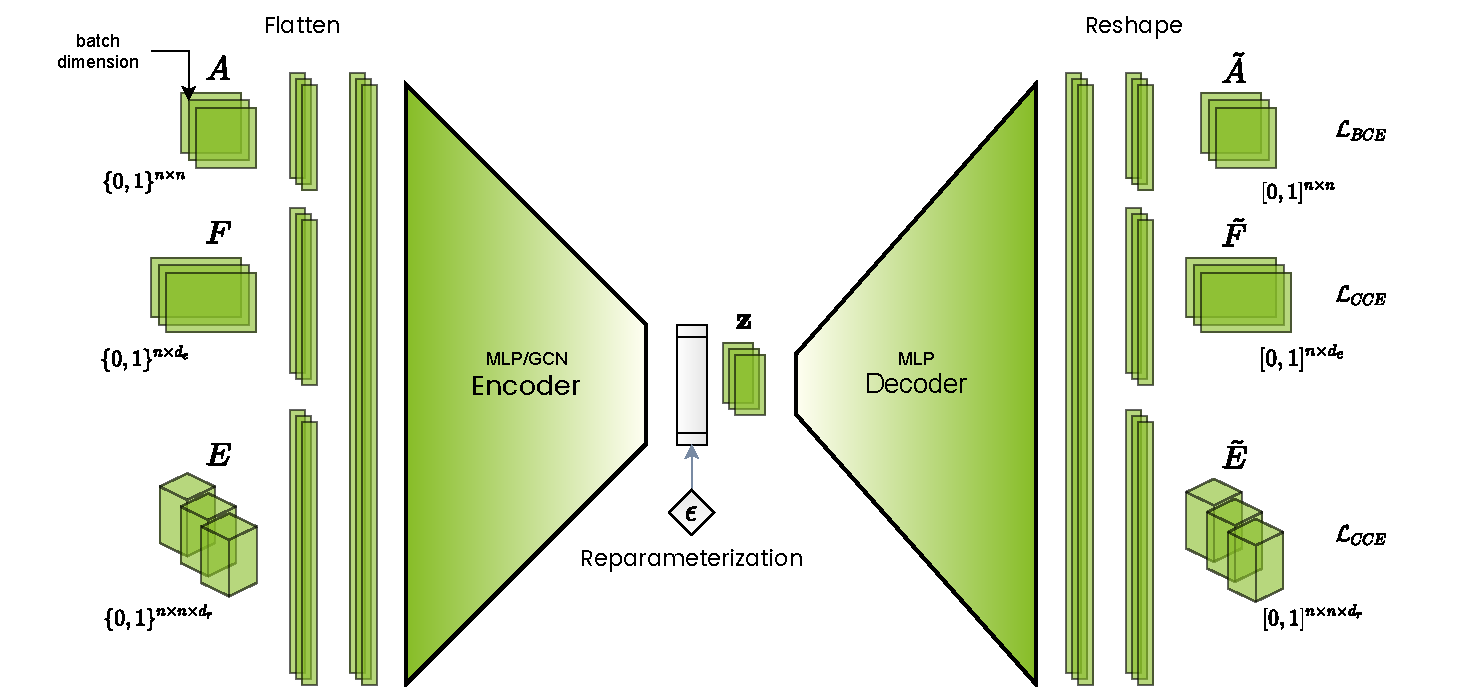
\includegraphics[scale=0.6,page=1]{data/images/rgvae_diagFull2.pdf}
    \caption{Architecture of the RGVAE.}
    \label{fig3:GVAE}
\end{figure}

% The encoder can either be a MLP, a GCNN or an RGCN. The same holds for the decoder with the addition that model architecture needs to be inverted. An version of a Graph VAE presented in \cite{simonovsky_graphvae_2018}. This model combines both the previous methods. The input graph undergoes relational graph convolutions before it is flattened and projected into latent space. After applying the reparametrization trick, a simple MLP decoder is used to regenerate the graph. In addition the model concatenates the input with a target vector $y$, which represents ???. The same vector is concatenated with the latent tensor. ***Elborate why they do that***.

% Reverse MLP

% Loss function

% What information can you capture when sparse compared to dense?


% Graphs can be generated recursively or in an one-shot approach. This paper uses the second approach and generates the full graph in one go. ***Cite?***
% This model be the starting point for our research.

% \subsubsection{One Shot vs. Recursive}
% One shot: MNIST vs recursive on graphs: Belli
In figure \ref{fig3:GVAE} the concept of the RGVAE is displayed. Each datapoint $G(A,E,F)$ is a subgraph from the KG dataset. Note that the model propagates batches instead of single datapoints. The RGVAE can generate graphs $\tilde{G}(\tilde{A},\tilde{E},\tilde{F})$ by sampling from the approximated posterior distribution $p_{{\theta}}\left G \mid \mathbf{z}\right)$. Since it predicts on closed sets of relations and entities, the generated subgraphs are either unseen and complement the KG or are already present in the dataset. The subgraph are sparse with $n$ nodes. A single triple being $n=2$ and a subgraph representation $2<n<40$, where $n=40$ was the explored maximum for the GraphVAE \cite{simonovsky_graphvae_2018}.  

\subsection{Graph Matching}
\label{ssec:graphmatch}

% Intro to graph matching on sparse graphs.
In this subsection we explain the term permutation invariance and its impact on the RGVAE's loss function. Further we present a $k$-factor graph matching algorithm for general graphs with edge and node attributes and the Hungarian algorithm as solution for the NP-hard problem of linear sum assignment. Finally we derive the full loss of the RGVAE when applying the calculated permutation matrix to the models prediction.

\subsubsection{Permutation Invariance}

% Permutation Invariance
% The position or rotation of a graph can vary. 
% Use graph matching to detect similarities between graphs

A visual example of permutation invariance is the image generation of numbers. If the loss function of the model would not be permutation invariant, the generated image could show a perfect replica of the input number, but being translated by one pixel the loss function would penalize the model. Geometrical permutations can be translation, scale or rotation around any axis. 

In the context of sparse graphs the most common, and relevant permutation for this thesis, is the position of a link in the adjacency matrix. By altering its position through matrix-multiplication of the adjacency and the permutation matrix, the original link can change direction or turn into a self-loop. When matching graphs with more $n>2$, permutation can change the nodes which the link connects. Further it is possible to match graphs only on parts of the graph, $k$-factor, instead of the full graph. In the case of different node counts between target and prediction graph, the target graph can be fully (1-factor) matched with the larger prediction graph. 

In context of this thesis, a model or a function is called permutation invariant, if it can match any permutation of the original. This allows the model a wider spectrum of predictions instead of penalizing it on the element-wise correct prediction of the adjacency.

% OR: An example is in object detection in images. An object can have geometrical permutations such as translation, scale or rotation, none the less the model should be able to detect and classify it. In that case, the model is not limited by permutations and  is there fore permutation invariant.
% In our case the object is a graph and the nodes can take different positions in the adjacency matrix. To detect similarities between graphs we apply graph matching.

\subsubsection{Max-Pool Graph matching algorithm}
% These are three of the state of the art graph matching algorithms.

% \begin{itemize}
%     \item Wasserstein
%     \item Maxpooling
%     \item one more
% \end{itemize}

Graph matching of general (not bipartite) graphs is a nontrivial task. Inspired by Simonovsky's approach \cite{simonovsky_graphvae_2018}, the RGVAE uses the max-pool algorithm, which can be effectively integrated in its loss function. Presented in \cite{cho_finding_2014} in the context of computer vision and successful in matching feature point graphs in an image. It first calculates the affinity between two graphs, considering node and edge attributes, then applies edge-wise max-pooling to reduce the affinity matrix to a similarity matrix. Cho \textit{et al.} praise the max-pool graph matching algorithm as resilient to deformations and highly tolerant to outliers compared to the mean or sum alternatives. The output is a normalized similarity matrix in continuous space of the same shape as the target adjacency matrix, indicating the similarity between each node of target and prediction graph. The similarity matrix is subtracted from a unit matrix to receive the cost matrix, necessary for the final step in the graph matching pipeline. Notable is, that this algorithm also allows $k$-factor matching, with $k \leq 1 < n$. Thus, subgraphs with different number of nodes can be matched. The final permutation matrix is determined by linear sum assignment of the cost matrix, a np-hard problem \cite{diestel2016graph}.

% Max-pooling algorithm comes here !!!
We use the previously presented sparse representation for subgraphs, sampled from a KG. The discrete target graph is $G=(A, E, F)$ and the continuous prediction graph $\widetilde{G}=(\widetilde{A}, \widetilde{E}, \widetilde{F})$. The $A, E, F$ matrices store the discrete data for the adjacency, for node attributes and the node attribute matrix of form $A \in\{0,1\}^{n \times n}$ with $n$ being the number of nodes in the target graph. $E\in\{0,1\}^{n \times n \times d_e}$ is the edge attribute matrix and a node attribute tensor of the shape $F\in\{0,1\}^{n \times d_n}$ with $d_e$ and $d_n$ being the size of the entity and relation dictionary. For the predicted graph with $k$ nodes, the adjacency matrix is $\widetilde{A} \in[0,1]^{k \times k}$, the edge attribute matrix is $\widetilde{E} \in \mathbb{R}^{k \times k \times d_{e}}$ and the node attribute matrix is $\widetilde{F} \in \mathbb{R}^{k \times d_{n}}$.


Given these graphs the algorithm aims to find the affinity matrix $S:(i, j) \times(a, b) \rightarrow \mathbb{R}^{+}$ where $i, j \in G$ and $a, b \in \widetilde{G}$. The affinity matrix returns a score for all node and all edge pairs between the two graphs and is calculated 

\begin{equation}
    \begin{array}{l}
        S((i, j),(a, b)) = \left(E_{i, j, \cdot}^{T}, \widetilde{E}_{a, b, \cdot}\right) A_{i, j} \widetilde{A}_{a, b} \widetilde{A}_{a, a} \widetilde{A}_{b, b}[i \neq j \wedge a \neq b] + \left(F_{i, \cdot}^{T} \widetilde{F}_{a, \cdot}\right) \widetilde{A}_{a, a}[i=j \wedge a=b].
    \end{array}
\label{eq3:s}
\end{equation}

Here the square brackets define Iverson brackets \cite{simonovsky_graphvae_2018}.


While affinity scores resemblances which suggest a common origin, similarity directly refers to the closeness between two nodes.
The next step is to find the similarity matrix $X^* \in[0,1]^{k \times n}$. 
Therefore we iterate a first-order optimization framework and get the update rule

\begin{equation}
    X^*_{t+1} \leftarrow \frac{1}{\left\|\mathbf{S} X^*_{t}\right\|_{2}} \mathbf{S} X^*_{t}.
\end{equation}

To calculate $\text { SX^* }$ we find the best candidate $X^*_{i,a}$ from the possible pairs of $i \in \mathbb{N}^{[0,n]}$ and $ai \in \mathbb{N}^{[0,k]}$ in the affinity matrix $S$. Heuristically, taking the argmax over all neighboring node pair affinities yields the best result. Other options are sum-pooling or average-pooling, which do not discard potentially irrelevant information, yet have shown to perform worse. Thus, using the max-pooling approach, we can pairwise calculate

\begin{equation}
    \mathbf{Sx}_{i a}=X^*_{i a} \mathbf{S}_{i a ; i a}+\sum^{n}_{j = 0}} \max _{0 \leq b < k \mathbb{N}_{a}} X^*_{j b} \mathbf{S}_{i a ; j b}.
\end{equation}

Depending on the matrix size, the number of iterations are adjusted. The resulting similarity matrix $X*$ yields a normalized similarity score for every node pair. The next step if to converting it to a discrete permutation matrix.



\subsubsection{Hungarian algorithm}
\label{ssec3:hung}

%  Find shortest path
Starting with the normalized similarity matrix $X^*$, we reformulate the aim of finding the discrete permutation matrix as a linear assignment problem. Simonovsky \textit{et al.} \cite{silver_mastering_2017}use for this purpose an optimization algorithm, the so called Hungarian algorithm. It original objective is to optimally assign $n$ resources to $n$ tasks, thus $k-n$ rows of the permutation matrix are left empty. The cost of assigning task $i \in \mathbb{N}^{[0,n]}$ to $a \in \mathbb{N}^{[0,k]}$ is stored in $x_{ia}$ of the cost matrix $C \in \mathbb{N}^{n \times k}$. By assuming tasks and resources are nodes and taking $C=1-X^*$ we get the continuous cost matrix $C$. This algorithm has a complexity of $O\left(n^{4}\right)$, thus is not applicable to complete KGs but only to subgraphs with limited number of nodes per graph \cite{date_gpu-accelerated_2016}.

The core of the Hungarian algorithm consist of four main steps, initial reduction, optimality check, augmented search and update. The presented algorithm is a popular variant of the original algorithm and improves the complexity of the update step from $O\left(n^{2}\right)$ to $O\left(n\right)$ and thus, reduces the total complexity to $O\left(n^{3}\right)$. Since throughout this thesis $n=k$ we imply the reduction step and continue with a quadratic cost matrix $C$. The following notation is solely to derive the Hungarian algorithm and does not apply to our graph data. The algorithm takes as input a bipartite graph $G=(V, U, E)$ and the cost matrix $C \in \mathbb{R}^{n \times n}$. $G$ bipartite because it considers all possible edges in the cost matrix in one direction and no self-loops. $V \in \mathbb{R}^n$ and $U \in \mathbb{R}^n$ are the resulting sets of nodes and $E \in \mathbb{R}^{n}$ the set of edges between the nodes. The algorithm's output is a discrete matching matrix $M$. To avoid two irrelevant pages of pseudocode, the steps of the algorithm are presented in the following short summary \cite{mills-tettey_dynamic_nodate}.

\begin{enumerate}
    \item Initialization: \\
    \begin{enumerate}
        \item Initialize the empty matching matrix $M_{0}=\emptyset$.
        \item Assign $\alpha_i$ and $\beta_i$ as follows:
        \begin{align*}
            \forall v_{i} &\in V, \quad &&\alpha_{i}=0 \\
            \forall u_{i} &\in U, \quad &&\beta_{j}=\min _{i}\left(c_{i j}\right)
        \end{align*}
        \end{enumerate}
    \item Loop $n$ times over the different stages:
    \begin{enumerate}
        \item Each unmatched node in $V$ is a root node for a Hungarian tree with completed results in an augmentation path.
        \item Expand the Hungarian trees in the equality subgraph. Store the indices $i$ of $v_i$ encountered in the Hungarian tree in the set $I*$ and similar for $j$ in $u_j$ and the set $J^*$. If an augmentation path is found, skip the next step.
        \item Update $\alpha$ and $\beta$ to add new edges to the equality subgraph and redo the previous step.
        \begin{align*}
            \theta&=\frac{1}{2} \min _{i \in I^{*}, j \notin J^{*}}\left(c_{i j}-\alpha_{i}-\beta_{j}\right) \\
            \alpha_{i} &\leftarrow\left\{\begin{array}{ll}
            \alpha_{i}+\theta & i \in I^{*} \\
            \alpha_{i}-\theta & i \notin I^{*}
            \end{array}\right \\
            \beta_{j} &\leftarrow\left\{\begin{array}{ll}
            \beta_{j}-\theta & j \in J^{*} \\
            \beta_{j}+\theta & j \notin J^{*}
            \end{array}\right \\
        \end{align*}
        \item Augment $M_{k-1}$ by flipping the unmatched with the matched edges on the selected augmentation path. Thus $M_k$ is given by $\left(M_{k-1}-P\right) \cup\left(P-M_{k-1}\right)$ and $P$ is the set of edges of the current augmentation path.
    \end{enumerate}
    \item Output $M_n$ of the last and $n^{th}$ stage.
\end{enumerate}



\subsubsection{Graph Matching VAE Loss}
\label{ssec3:GVAEloss}
Coming back to our generative model, we now explain how the loss function needs to be adjusted to work with graphs and graph matching, which results in a permutation invariant graph VAE.

The normal VAE maximizes the evidence lower-bound or, in a practical implementation, minimizes the upper-bound on negative log-likelihood. Using the notation of section \ref{ssection:VAE} the graph VAE loss is

\begin{equation}
    \begin{array}{l}
    \mathcal{L}(\phi, \theta ; G)=\mathbb{E}_{q_{\phi}(\mathbf{z} \mid G)}\left[-\log p_{\theta}(G \mid \mathbf{z})\right]+\beta (\operatorname{KL}\left[q_{\phi}(\mathbf{z} \mid G) \| p(\mathbf{z})\right]).
    \end{array}
\end{equation}

The loss function $\mathcal{L}$ is a combination of reconstruction term and regularization term. The regularization term is the KL divergence between a standard normal distribution and the latent space distribution of $\mathbf{z}$. The change to graph data does not influence this term  to graphs. The reconstruction term is the cross entropy between prediction and target, binary for the adjacency matrix and categorical for the edge and node attribute matrices. 

% A sigmoid with logits, E,F, softmax include translation X

% r. Sigmoid activation function is used to compute
% Ae, whereas edge- and node-wise softmax is applied to obtain
% Ee and Fe, respectively. A

The predicted output of the decoder is split in three parts and while $\tilde{A}$ is activated through sigmoid, $\tilde{E}$ and $\tilde{F}$ are activated via edge- and nodewise Softmax. 
For the case of $n<k$, the target adjacency is permuted $A^{\prime}=X A X^{T}$, so that the model can backpropagate over the full prediction. Since $E$ and $F$ are categorical, permuting prediction or target yields the same cross-entropy. Following Simonovsky's approach \cite{simonovsky_graphvae_2018} we permute the prediction, $\widetilde{F}^{\prime}=X^{T} \widetilde{F}$ and $\widetilde{E}_{\cdot, \cdot, l}^{\prime}=X^{T} \widetilde{E}_{\cdot, \cdot, l} X$. Let $l$ be the one-hot encoded edge attribute vector which is permuted. These permuted subgraphs are then used to calculate the maximum log-likelihood estimate \cite{simonovsky_graphvae_2018}:

\begin{equation}
    \begin{split}
        \log p\left(A^{\prime} \mid \mathbf{z}\right) = &1 / k \sum_{a} A_{a, a}^{\prime} \log \widetilde{A}_{a, a}+\left(1-A_{a, a}^{\prime}\right) \log \left(1-\widetilde{A}_{a, a}\right)+ \\ & +1 / k(k-1) \sum_{a \neq b} A_{a, b}^{\prime} \log \widetilde{A}_{a, b}+\left(1-A_{a, b}^{\prime}\right) \log \left(1-\widetilde{A}_{a, b}\right)
    \end{split}
    \label{eq3:GAVElossA}
\end{equation}

\begin{align}
    \log p(F \mid \mathbf{z}) &=1 / n \sum_{i} \log F_{i, \cdot}^{T} \widetilde{F}_{i,}^{\prime} \\
    \log p(E \mid \mathbf{z}) &=1 /\left(\|A\|_{1}-n\right) \sum_{i \neq j} \log E_{i, j,}^{T}, \widetilde{E}_{i, j, \cdot}^{\prime}
    \label{eq3:GAVElossEF}
\end{align}

The normalizing constant $1 / k(k-1)$ takes into account the no self-loops restriction, thus an edge-less diagonal. In the case of self loops this constant is $1 / k^2$. Similar $1 /\left(\|A\|_{1}-n\right)$ for $\log p(E \mid \mathbf{z})$ where $-n$ accounts for the edge-less diagonal and in case of self-loops is discarded, resulting in $1 /\left(\|A\|_{1}\right)$.

\subsection{Ranger Optimizer}
\label{sec3:ranger}

Finalizing this chapter, we explain the novel deep learning optimizer Ranger. Ranger combines Rectified Adam (RAdam), lookahead and optionally gradient centralization. Let us briefly look into the different components.
RAdam is based on the popular Adam optimizer. It improves the learning by dynamically rectifying Adam's adaptive momentum. This is done by reducing the variance of the momentum, which is especially large at the beginning of the training. Thus, leading to a more stable and accelerated start \cite{liu_variance_2020}.
The Lookahead optimizer was inspired by recent advances in the understanding of loss surfaces of deep neural networks, thus proposes an approach where, a second optimizer estimates the gradients behavior for the next steps on a set of parallel trained weights, while the number of 'looks ahead' steps is a hyperparameter.
This improves learning and reduces the variance of the main optimizer \cite{zhang_lookahead_2019}.
The last and most novel optimization technique, Gradient Centralization, acts directly on the gradient by normalizing it to a zero mean. Especially on convolutional neural networks, this helps regularizing the gradient and boosts learning. This method can be added to existing optimizers and can be seen as constrain of the loss function \cite{yong_gradient_2020}.
Concluding we can say that Ranger is a state of the art deep learning optimizer with accelerating and stabilizing properties, incorporating three different optimization methods, which synergize with each other. Considering that generative models are especially unstable during training, we see Ranger as a good fit for this research.



% LookAhead was inspired by recent advances in the understanding of loss surfaces of deep neural networks, and provides a breakthrough in robust and stable exploration during the entirety of training.